\chapter{Extendiendo el borrow checker}

\section{Entendiendo los procesos del compilador}

El compilador de Rust según \cite{rustcdevelopment} se diferencia del resto, ya que hace procesos que otros no realizan (borrow-checking) y también toma algunas decisiones no convencionales. El proceso de compilación de un programa comienza al invocar el comando \textbf{rustc} junto al código fuente de un programa y los parámetros. El modulo \textit{rustc\_driver} se encarga de captar los argumentos y definir la configuración que se utilizará en el resto del procedimiento.

Una vez que el compilador captó el código, los módulos \textit{rustc\_lexer} y \textit{rustc\_parse} se encargan de analizarlo y generar el AST (árbol de sintaxis abstracta). En esta primera etapa también se expanden las macros, se resuelven los nombres, se chequea la sintaxis del programa y se valida que el AST sea correcto.

\begin{wrapfigure}{r}{0.25\textwidth}
    \caption{Compiler pipeline}
    \centering
    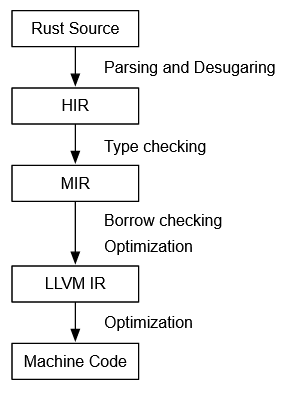
\includegraphics[width=0.3\textwidth]{compiler-flow}
\end{wrapfigure}

Teniendo este árbol, se proceden a generar las representaciones intermedias. La primera en construirse es el HIR ( High-Level Intermediate Representation) que es una version más amigable para el compilador del AST. Durante este proceso se realiza la inferencia de tipos, la resolución de las traits y principalmente el chequeo de tipos, donde se convierten los tipos encontrados en el HIR por representaciones internas usadas por el compilador. Estas son usadas para aumentar la seguridad, correctitud y coherencia de los tipos utilizados en el programa.

La siguiente parte es la construcción del MIR (Mid-Level Intermediate Representation) a partir del HIR. Aquí es donde se hacen gran parte de las optimizaciones del código, junto al pattern-matching y chequeos de exhaustividad. Además, el MIR es donde se realiza el \text{borrow-checking} y otros chequeos importantes basados en el flujo de datos. Debido a que es una representación de alto nivel y genérica es aquí donde se realizan la mayoría de análisis del compilador, y nosotros tomaremos en cuenta esto para añadir nuestros propios algoritmos y análisis.

A continuación se realiza lo que es conocido por la generación de código o \textit{codegen}, que consiste en transformar las representaciones de alto nivel a un binario executable. \textbf{rustc} utiliza \textbf{LLVM} para esto. Se comienza convirtiendo el MIR en LLVM IR (LLVM Intermediate Representation) para luego pasárselo a LLVM, el cual realiza más optimizaciones, y emitir el código de maquina. Este es básicamente código assembler con algunos tipos y anotaciones añadidos. Los diferentes binarios/bibliotecas luego son unidos (linked) para crear el binario final.

\section{Análisis estáticos sobre el MIR}

\subsection{MIR}

\cite{rustcdevelopment} dice el MIR que es una forma simplificada de Rust el compilador utiliza principalmente para comprobaciones de seguridad flow-sensitive, como por ejemplo el borrow checker. Esta definido en el modulo \textbf{rust\_middle::mir}, se basa en un CFG (Control-Flow Graph o Grafo de Control de Flujo) y todos los tipos son explícitos.

El CFG es un término común en el ámbito de los compiladores, ya que permite representar un programa exponiendo de manera clara el flujo del mismo. El CFG del MIR esta estructurado como un conjunto de bloques básicos conectados por aristas. Estos bloques básicos están conformados por un conjunto de \textit{statements} que se ejecutarían juntos y de manera secuencial y completa. Al final se encuentra un \textit{terminator} cuya función es referenciar y conectar bloques básicos. La construcción de un CFG es generalmente el primer paso de la mayoría de los algoritmos de análisis flow-sensitive, y el MIR esta estructurado de esta manera para facilitar estos análisis.

Otros conceptos claves del MIR son:
\begin{itemize}
    \item \textbf{Locals}: Lugar de la memoria alojado (conceptualmente) en el stack. Se representan con un guion bajo seguido de un numero, por ejemplo \_1. El lugar \_0 esta reservado para la dirección de retorno de la función.
    \item \textbf{Places}: Expresiones que identifican un lugar en la memoria.
    \item \textbf{Rvalues}: Expresiones que producen un valor. Su nombre proviene del hecho de que están del lado derecho de una asignación.
    \begin{itemize}
        \item \textbf{Operands}: Son los argumentos de un rvalue, que pueden ser constantes o Places
    \end{itemize}
\end{itemize}

Mediante el uso de las versiones nightly del compilador, que añaden la posibilidad de importar módulos críticos e imperativos para los análisis estáticos que queremos realizar, es posible acceder y utilizar las distintas representaciones intermedias de un código fuente.

Podemos apreciar la transformación a MIR mediante un ejemplo. El siguiente programa básico
\begin{lstlisting}[language=Rust]
    fn main() {
        let mut x = 5;
        x = x + 10;
    }
\end{lstlisting}
tiene una representación en MIR de la siguiente forma:
\begin{lstlisting}[language=Rust]
    // WARNING: This output format is intended for human consumers only
    // and is subject to change without notice. Knock yourself out.
    fn main() -> () {
        let mut _0: ();            // return place in scope 0 at ./examples/simple_sum.rs:1:11: 1:11
        let mut _1: i32;           // in scope 0 at ./examples/simple_sum.rs:2:9: 2:14
        scope 1 {
            debug x => _1;                   // in scope 1 at ./examples/simple_sum.rs:2:9: 2:14
        }

        bb0: {
            _1 = const 5_i32;      // scope 0 at ./examples/simple_sum.rs:2:17: 2:18
            _1 = const 15_i32;     // scope 1 at ./examples/simple_sum.rs:3:5: 3:15
            return;                // scope 0 at ./examples/simple_sum.rs:4:2: 4:2
        }
    }
\end{lstlisting}

Este ejemplo, como indica el comentario arriba, muestra el MIR para que sea más sencillo de leer por las personas. Podemos apreciar como se crea la función main, se realizan las declaraciones de las variables en la parte superior y luego procede a definirse los bloques básicos. En este caso, el bloque bb0 es el único que se construyo y contiene dos statements y un terminator. Debido a la optimizaciones del compilador (expansión de constantes), los statements son solo asignaciones directas sin la necesidad de hacer una suma como en el programa fuente. El terminator en este caso es la llamada a return.

Para extender el borrow checker, se realiza una interpretación abstracta del MIR aplicando los análisis estáticos necesarios y recopilando la información.

\subsection{Stacked borrows}

Stacked Borrows \cite{stackedborrows} propone una semántica operacional para los accesos de memoria en Rust que refuerza. Stacked borrows define una disciplina de aliasing y declara que cualquier programa que la viole contendrá comportamiento no definido, lo que significa que el compilador puede descartarlos a la hora de realizar optimizaciones. Esto lo realiza introduciendo condiciones claramente definidas en las cuales un programa Rust no se comporta debidamente debido a un error de aliasing. La idea es definir una version dinámica del \textit{borrow-checker} que Rust ya utiliza para comprobar que los accesos se hagan de acuerdo a la política de aliasing.

El borrow checker en particular comprueba que las referencias que puedan superponerse, se utilicen de una manera bien anidada. Stacked Borrows modela esta disciplina mediante un análisis haciendo uso de una pila por locación: se detecta cuando las referencias no son utilizadas que sigan el método de pila, y se marca a esos programas como erroneos. Basados en eso, se extiende Stacked Borrows para las reglas de los punteros planos (que son ignorados por el borrow-checker) con el objetivo de ser lo más liberes posibles sin interferir con las propiedades principales de un "fragmento seguro" del análisis que realizan.

La idea principal detrás de Stacked Borrows es tomar el análisis estático que realiza el borrow checker, el cual utiliza lifetimes, y transformarlo en un análisis dinámico el cual no haga uso de lifetimes. De esta manera, se puede lograr que inclusive aquellos programas que contengan unsafe deban satisfacer esta comprobación. Los programas Safe deberían trivialmente satisfacer el nuevo chequeo, ya que este es estrictamente mas libre que el anterior.

De manera simplificada, la version dinámica del borrow checker debería asegurar que:
\begin{enumerate}
    \item Una referencia y todas las referencias derivadas de esta puedan ser usadas solamente durante su lifetime, y
    \item El referente no es utilizado hasta que el lifetime del préstamo haya expirado.
\end{enumerate}

Consideremos el ejemplo brindado por \cite{stackedborrows}:
\begin{lstlisting}[language=Rust]
1 let mut local = 0;
2 let x = & mut local ;
3 let y = & mut *x;   // Reborrow x to y.
4 *x = 1;             // Use x again.
5 *y = 2;             // Error ! y used after x got used
\end{lstlisting}

Este programa viola el principio de la debido a un uso de la referencia \textit{y} que ocurre en la linea 5 despues del siguiente uso del referente \textit{x} en la linea 4, y por lo tanto este programa es rechazado por el borrow-checker. Si observamos el patron de uso, podemos observar que ``XYXY'' es una violación a la idea de anidación. Para que el programa sea conforme con la política de la pila, debería tener los accesos anidados de la manera ``XYYX''.

Para llevar esta idea a cabo, Stacked Borrows define un modelo operacional. Primero se debe ser capaz de distinguir las referencias que apuntan a un mismo lugar de la memoria; por eso se asume que todas las referencias son marcadas con un ID único cuando son creadas, y este se preserva a medida que la referencia es copiada. Luego, en memoria se debe almacenar una pila que almacenará los IDs de las referencias junto a información para distinguir el tipo de item (Unique, SharedReadOnly o SharedReadWrite) que es.

Las principales reglas del modelo son las siguientes:
\begin{itemize}
    \item (new-mutable-ref) Cada vez que una nueva referencia mutable es creada (\&mut expr) de algún valor referente existente, primero que nada se considera \textit{uso} de ese referente. Luego se elige un ID nuevo para la referencia, y se la coloca junto a su tipo (Unique) en el tope de la pila.
    \item (new-mutable-raw) Cada vez que una variable mutable plana (raw pointer) es creada mediante un casteo (expr as \*mut T) a partir de una referencia mutable (\&mut T) con el valor de algun referente, primero es considerada un uso de esa referencia mutable. Luego se añade la referencia del tipo SharedReadWrite al tope de la pila.
    \item (new-shared-ref) Cada vez que una nueva referencia compartida es creada (\&expr) a partir de un valor existente de un referente, primero es considerado un \textit{acceso de lectura} del valor. Luego se elige un ID nuevo para la referencia, y se la coloca junto a su tipo SharedReadOnly en el tope de la pila.
    \item (uso) Cada vez que un referente X es utilizado, un item con el ID X debe estar en la pila. Si existen otros items por encima de este, hay que removerlos, de tal manera que X quede en el tope de la pila. En el caso de que la pila no contenga ningún item Unique con el mismo ID del referente usado, o un valor SharedReadOnly o SharedReadWrite, entonces el programa tiene comportamiento no deseado.
    \item (lectura) Cada vez que una referencia X es leida, un item con el ID X debe encontrarse en la pila. Se remueven los elementos del tope de la pila hasta que todos los items por encima de X son SharedReadOnly. Si no existe ningún item con ID X en la pila, el programa viola el modelo planteado.
\end{itemize}

Existen ciertas extensiones y optimizaciones que pueden realizarse a este modelo, sin embargo estas son las reglas que consideramos mínimas para detectar errores de aliasing en la mayor parte de programas y son las que implementaremos en la herramienta.

Stacked borrows fue definido formalmente y esta verificado utilizando Coq. Además, como hemos mencionado el interprete MIRI \cite{miri} dentro de las variedades de chequeos que realiza, posee una implementación bastante robusta del modelo de Stacked Borrows donde se pueden realizar tests para comprobar su utilidad.